\begin{surferPage}[Singularidad A4+-]{Una singularidad $A_4^{+-}$}
Una $A_4^{+-}$ es parecida a cualquier singularidad de tipo
$A_{2k}^{+-}$, $k\ge 1$, como se ve mirando la ecuación
    \[x^{2k+1}+y^2-z^2=0.\]
La única diferencia aparente con una
$A_2^{+-}$ (imagen abajo a la izquierda)
es el orden de tangencia. La otras dos imágenes son
de una $A_4^{+-}$ y una $A_6^{+-}$), respectivamente.
    \vspace*{-0.5em}
    \begin{center}
      \begin{tabular}{c@{\quad}c@{\quad}c}
        \begin{tabular}{@{}c@{}}
          
\includegraphics[width=1.2cm]{../../common/images/A2pm}
        \end{tabular}
        &
        \begin{tabular}{@{}c@{}}
          
\includegraphics[width=1.2cm]{../../common/images/A4pm}
        \end{tabular}
        &
        \begin{tabular}{@{}c@{}}
          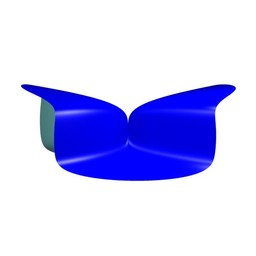
\includegraphics[width=1.2cm]{../../common/images/A6pm}
        \end{tabular}
      \end{tabular}
    \end{center}
    \vspace*{-0.4em}
Pero ello proporciona una diferencia fundamental con la deformación a
singularidades cónicas. Lo ilustramos con
una deformación en una superficie con agujeros.
Para una $A_k^{+-}$, se pueden obtener $k$ agujeros, 4 en
nuestro caso (en la imagen se ven en dos pares;
comparar con el caso de $A_2^{+-}$, con un agujero, ya visto antes).
    \begin{center}
      \vspace{-0.1cm}
      \begin{tabular}{@{}c@{\quad}c@{}}
        \begin{tabular}{@{}c@{}}
          
\includegraphics[width=1.2cm]{../../common/images/A4pm_sm_0}
        \end{tabular}
        &
        \begin{tabular}{@{}c@{}}
          
\includegraphics[width=1.2cm]{../../common/images/A4pm_sm_1}
        \end{tabular}
      \end{tabular}
    \end{center}
%     \dontshow{
%     %
%     \begin{center}
%       \vspace{-0.1cm}
%       \begin{tabular}{@{}c@{\quad}c@{\quad}c@{}}
%         \begin{tabular}{@{}c@{}}
%           
\includegraphics[width=1.2cm]{../../common/images/A4pm_0}
%         \end{tabular}
%         &
%         \begin{tabular}{@{}c@{}}
%           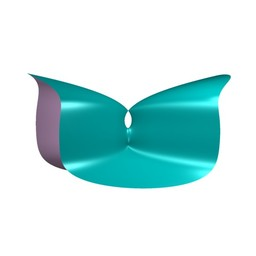
\includegraphics[width=1.2cm]{../../common/images/A4pm_1}
%         \end{tabular}
%         &
%         \begin{tabular}{@{}c@{}}
%           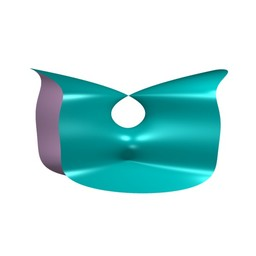
\includegraphics[width=1.2cm]{../../common/images/A4pm_2}
%         \end{tabular}
%       \end{tabular}
%     \end{center}
%     }
 
\end{surferPage}
